\begin{figure}[!]%[!ht]
	\centering
\begin{tikzpicture}[thick,scale=0.55, every node/.style={transform shape}] 
\tikzstyle{every loop}=[]
\node[style={circle,draw,thick,align=center, fill={black}, minimum size=1cm},pattern=dots] (1) at (2.8284, 2.8284) {}; 
\node[style={circle,draw,thick,align=center, fill={black}, minimum size=1cm},pattern=dots] (2) at (4, 0) {};
\node[style={circle,draw,thick,align=center, fill={white}, minimum size=1cm}] (3) at (2.8284, -2.8284) {}; 
\node[style={circle,draw,thick,align=center, fill={white}, minimum size=1cm}] (4) at (0, -4) {};
\node[style={circle,draw,thick,align=center, fill={black}, minimum size=1cm},pattern=dots] (5) at (-2.8284, -2.8284) {}; 
\node[style={circle,draw,thick,align=center, fill={white}, minimum size=1cm}] (6) at (-4, 0) {}; 
\node[style={circle,draw,thick,align=center, fill={black}, minimum size=1cm},pattern=dots] (7) at (-2.8284, 2.8284) {};
\node[style={circle,draw,thick,align=center, fill={white}, minimum size=1cm}] (8) at (0,4) {};


  \foreach \angle in {30,60,...,150}
    {\pgfpathcircle{
    \pgfpointadd{\pgfpointpolar{\angle}{1.5cm}}{\pgfpoint{0cm}{4cm}}
    }{0.1cm}
    \draw[red, thick,-] (0,4) -- +(\angle:1.5);
    }
  \pgfusepath{fill};
  
    \foreach \angle in {210,240,...,330}
    {\pgfpathcircle{
    \pgfpointadd{\pgfpointpolar{\angle}{1.5cm}}{\pgfpoint{0cm}{-4cm}}
    }{0.1cm}
    \draw[red, thick,-] (0,-4) -- +(\angle:1.5);
    }
  \pgfusepath{fill};
  
  \foreach \angle in {100,120,140,160,180,200,220,240,260}
    {\pgfpathcircle{
    \pgfpointadd{\pgfpointpolar{\angle}{1.5cm}}{\pgfpoint{-4cm}{0cm}}
    }{0.1cm}
    \draw[red, thick,-] (-4,0) -- +(\angle:1.5);
    }
  \pgfusepath{fill};
  
    \foreach \angle in {300,320,340,0,20,40,60}
    {\pgfpathcircle{
    \pgfpointadd{\pgfpointpolar{\angle}{1.5cm}}{\pgfpoint{4cm}{0cm}}
    }{0.1cm}
    \draw[red, thick,-] (4,0) -- +(\angle:1.5);
    }
  \pgfusepath{fill};
  
  
      \foreach \angle in {190,210,230,250,270}
    {\pgfpathcircle{
    \pgfpointadd{\pgfpointpolar{\angle}{1.5cm}}{\pgfpoint{-2.8284cm}{-2.8284cm}}
    }{0.1cm}
    \draw[red, thick,-] (-2.8284, -2.8284) -- +(\angle:1.5);
    }
  \pgfusepath{fill};
  
        \foreach \angle in {270,290,310,330,350}
    {\pgfpathcircle{
    \pgfpointadd{\pgfpointpolar{\angle}{1.5cm}}{\pgfpoint{2.8284cm}{-2.8284cm}}
    }{0.1cm}
    \draw[red, thick,-] (2.8284,-2.8284) -- +(\angle:1.5);
    }
  \pgfusepath{fill};
  
          \foreach \angle in {110,130,150,170}
    {\pgfpathcircle{
    \pgfpointadd{\pgfpointpolar{\angle}{1.5cm}}{\pgfpoint{-2.8284cm}{2.8284cm}}
    }{0.1cm}
    \draw[red, thick,-] (-2.8284,2.8284) -- +(\angle:1.5);
    }
  \pgfusepath{fill};
  
            \foreach \angle in {10,30,50,70}
    {\pgfpathcircle{
    \pgfpointadd{\pgfpointpolar{\angle}{1.5cm}}{\pgfpoint{2.8284cm}{2.8284cm}}
    }{0.1cm}
    \draw[red, thick,-] (2.8284,2.8284) -- +(\angle:1.5);
    }
  \pgfusepath{fill};
  
\path[]
    (2) [-,blue,thick] edge node[above,minimum size=0pt] {} (5)
    (2) [-,blue,thick] edge node[above,minimum size=0pt] {} (7)
    (5) [-,blue,thick] edge node[right,minimum size=0pt] {} (7)
    (1) [-,blue,thick] edge node[right,minimum size=0pt] {} (2)
    (1) [-,blue,thick] edge node[right,minimum size=0pt] {} (5)
    (1) [-,blue,thick] edge node[right,minimum size=0pt] {} (7)
 ;   
\path[]
  %  (1) [-,dashed] edge node[above,minimum size=0pt] {} (2)
    (1) [-,dashed] edge node[above,minimum size=0pt] {} (3)
    (1) [-,dashed] edge node[below,minimum size=0pt] {} (4)
  %  (1) [-,dashed] edge node[right,minimum size=0pt] {} (5)
    (1) [-,dashed] edge node[above,minimum size=0pt] {} (6)
  %  (1) [-,dashed] edge node[below,minimum size=0pt] {} (7)
    (1) [-,dashed] edge node[right,minimum size=0pt] {} (8)
    (2) [-,dashed] edge node[above,minimum size=0pt] {} (3)
    (2) [-,dashed] edge node[above,minimum size=0pt] {} (4)
    (2) [-,dashed] edge node[above,minimum size=0pt] {} (6)
    (2) [-,dashed] edge node[above,minimum size=0pt] {} (8)
    (3) [-,dashed] edge node[above,minimum size=0pt] {} (4)
    (3) [-,dashed] edge node[above,minimum size=0pt] {} (5)
    (3) [-,dashed] edge node[below,minimum size=0pt] {} (6)
    (3) [-,dashed] edge node[right,minimum size=0pt] {} (7)
    (3) [-,dashed] edge node[right,minimum size=0pt] {} (8)
    (4) [-,dashed] edge node[above,minimum size=0pt] {} (5)
    (4) [-,dashed] edge node[above,minimum size=0pt] {} (6)
    (4) [-,dashed] edge node[below,minimum size=0pt] {} (7)
    (4) [-,dashed] edge node[right,minimum size=0pt] {} (8)
    (5) [-,dashed] edge node[right,minimum size=0pt] {} (6)
    (5) [-,dashed] edge node[above,minimum size=0pt] {} (8)
    (6) [-,dashed] edge node[below,minimum size=0pt] {} (7)
    (6) [-,dashed] edge node[right,minimum size=0pt] {} (8)
    (7) [-,dashed] edge node[right,minimum size=0pt] {} (8);
\filldraw[black] (-9.25,4.85) circle (0pt) node[anchor=west] {user};
\filldraw[black] (-9.25,3) circle (0pt) node[anchor=west] {node (not in committee)};
\filldraw[black] (-9.25,4) circle (0pt) node[anchor=west] {node (committee member)};

\node[style={circle,draw,thick,align=center, red, minimum size=0.1cm}] (10) 
at (-10, 4.85) {};
\node[style={circle,draw,thick,align=center, fill={white}, minimum size=0.9cm}] (11) 
at (-10, 3) {};
\node[style={circle,draw,thick,align=center, fill={black}, minimum size=0.9cm},pattern=dots] (12) at (-10, 4) {};
\draw (-10.85, 5.3) rectangle (-4.8, 2.3);

\end{tikzpicture}
 \caption{Illustration of a \name fully mesh network with $n=8$ nodes, serving various numbers of users. Among the nodes, $m=4$ nodes (filled with dots) participate in the committee of some term $r$.
}\label{fig_illustration_network}
\end{figure}

This section is dedicated to a high-level description of the Helix protocol---we first illustrate the main data types used in \name and then describe its operation.

In \nameNS, users issue \textbf{Encrypted-transactions} ($etx$s), which they send to the node they are connected to via a user-node connection. We refer to the receiving node as the \emph{owner} node of the $etx$. $etx$s are stored locally by every node in her \textbf{Epool}, pool of Encrypted-transactions. The protocol's goal is to order the $etx$s, such that the order is agreed upon by all correct nodes. The $etx$s are grouped into \textbf{Eblocks}, blocks of Encrypted-transactions, which will ultimately be incorporated into the blockchain. The protocol progresses in iterations, or \textbf{terms}, where in each term exactly one Eblock is appended to the blockchain. 

Agreement on the next Eblock in the blockchain is achieved using a Byzantine agreement protocol, run within a \textbf{committee} comprising a subset of the nodes (see Fig.~\ref{fig_illustration_network}). A special feature of \name is that the committee members constructing an Eblock do not know the content of the transactions or their owner nodes. This property is achieved by encrypting transactions using a $(t,n)$-threshold encryption scheme among the nodes, where $t=f$, and broadcasting them anonymously.
After a committee reaches an agreement on a new Eblock, a proof for this agreement, referred to as a \textbf{Block-proof}, is constructed and broadcasted to all nodes. Only then is the Eblock decrypted, in a process where, first each individual node produces her own \textbf{Shares-block}, and later $t+1$ (for a further explanation see Sec.~\ref{segment3}) different Shares-blocks are later combined to reveal the \textbf{Dblock}, block of decrypted $etx$s (corresponding to the Eblock).						

Each node incorporates a so-called \textbf{Encrypted-secret} into the Shares-block that she generates. When the Dblock is revealed (i.e., decrypted from the corresponding Eblock), the Encrypted-secrets are also decrypted, and combined together to generate an unpredictable \textbf{random seed}. This random seed is used, together with the \textbf{reputations} of the nodes, to determine the new committee members responsible for appending a new Eblock to the blockchain in the next term.
Intuitively, the reputation is a measure of node's behavior in the protocol.


\begin{figure*}
%[!b]%[!ht]
	\centering
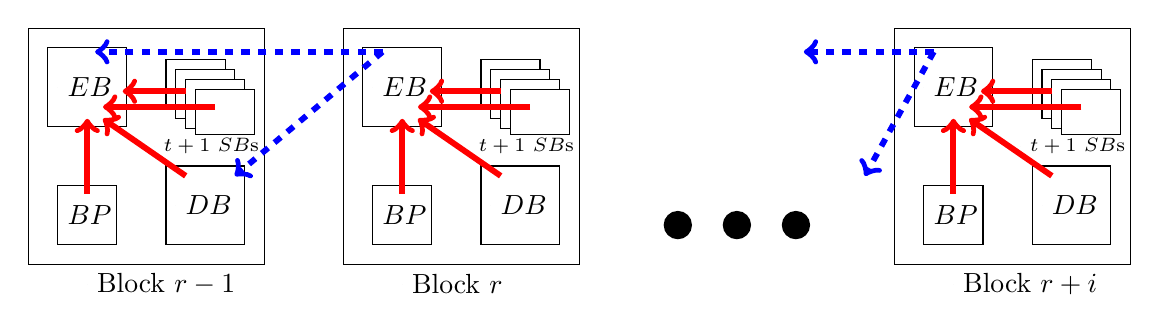
\begin{tikzpicture}
\tikzstyle{every loop}=[]
\draw (0,0) rectangle (3,3);
\draw (0.25,1.75) rectangle (1.25,2.75); %EB
\draw (1.75,0.25) rectangle (2.75,1.25); %DB
\draw (0.375,0.25) rectangle (1.125,1); %BP

\draw [fill=white] (1.75,1.975) rectangle (2.5,2.6);
\draw [fill=white] (1.875,1.85) rectangle (2.625,2.475);
\draw [fill=white] (2,1.725) rectangle (2.75,2.35);
\draw [fill=white] (2.125,1.65) rectangle (2.875,2.225);


\filldraw[black] (0.375,2.25) circle (0pt) node[anchor=west] {$EB$};
\filldraw[black] (1.875,0.75) circle (0pt) node[anchor=west] {$DB$};
\filldraw[black] (0.375,0.625) circle (0pt) node[anchor=west] {$BP$};
\filldraw[black] (1.6,1.5) circle (0pt) node[anchor=west] {\scriptsize$t+1$ $SB$s};
\filldraw[black] (0.75,-0.25) circle (0pt) node[anchor=west] {Block $r-1$};
\draw [->,solid,thick, red, line width=0.75mm] (0.75,0.9) to  (0.75,1.85);% Arrow
 \draw [->,solid,thick, red, line width=0.75mm] (2.375,2) to  (0.95,2);% Arrow   
  \draw [->,solid,thick, red, line width=0.75mm] (2,2.2) to  (1.20,2.2);% Arrow   
 \draw [->,solid,thick, red, line width=0.75mm] (2,1.125) to  (0.95,1.85); % Arrow

\draw (4,0) rectangle (7,3);
\draw (4.25,1.75) rectangle (5.25,2.75); %EB
\draw (5.75,0.25) rectangle (6.75,1.25); %DB
\draw (4.375,0.25) rectangle (5.125,1); %BP

\draw [fill=white] (5.75,1.975) rectangle (6.5,2.6);
\draw [fill=white] (5.875,1.85) rectangle (6.625,2.475);
\draw [fill=white] (6,1.725) rectangle (6.75,2.35);
\draw [fill=white] (6.125,1.65) rectangle (6.875,2.225);
\filldraw[black] (4.375,2.25) circle (0pt) node[anchor=west] {$EB$};
\filldraw[black] (5.875,0.75) circle (0pt) node[anchor=west] {$DB$};
\filldraw[black] (4.375,0.625) circle (0pt) node[anchor=west] {$BP$};
\filldraw[black] (5.6,1.5) circle (0pt) node[anchor=west] {\scriptsize$t+1$ $SB$s};
\filldraw[black] (4.75,-0.25) circle (0pt) node[anchor=west] {Block $r$};
\draw [->,solid,thick, red, line width=0.75mm] (4.75,0.9) to  (4.75,1.85);% Arrow
 \draw [->,solid,thick, red, line width=0.75mm] (6.375,2) to  (4.95,2);% Arrow   
  \draw [->,solid,thick, red, line width=0.75mm] (6,2.2) to  (5.10,2.2);% Arrow   
 \draw [->,solid,thick, red, line width=0.75mm] (6,1.125) to  (4.95,1.85); % Arrow
 \draw [->,dashed,thick, blue, line width=0.75mm] (4.5,2.7) to  (0.85,2.7);
  \draw [->,dashed,thick, blue, line width=0.75mm] (4.5,2.7) to  (2.625,1.125);
 
%  \draw [ultra thick,red] (-2,2) to[out=45,in=115] (1,1) to[out=-180+115,in=10] (-5,-3);
%\draw (0,0) to[out=90,in=180] (3,2);

\node[style={circle,draw,thick,align=center, fill={black}}] (0) at (8.25, 0.5) {};
\node[style={circle,draw,thick,align=center, fill={black}}] (0) at (9, 0.5) {};
\node[style={circle,draw,thick,align=center, fill={black}}] (0) at (9.75, 0.5) {};


\draw (11,0) rectangle (14,3);
\draw (11.25,1.75) rectangle (12.25,2.75); %EB
\draw (12.75,0.25) rectangle (13.75,1.25); %DB
\draw (11.375,0.25) rectangle (12.125,1); %BP

\draw [fill=white] (12.75,1.975) rectangle (13.5,2.6);
\draw [fill=white] (12.875,1.85) rectangle (13.625,2.475);
\draw  [fill=white] (13,1.725) rectangle (13.75,2.35);
\draw [fill=white] (13.125,1.65) rectangle (13.875,2.225);

\filldraw[black] (11.375,2.25) circle (0pt) node[anchor=west] {$EB$};
\filldraw[black] (12.875,0.75) circle (0pt) node[anchor=west] {$DB$};
\filldraw[black] (11.375,0.625) circle (0pt) node[anchor=west] {$BP$};
\filldraw[black] (12.6,1.5) circle (0pt) node[anchor=west] {\scriptsize$t+1$ $SB$s};
\filldraw[black] (11.75,-0.25) circle (0pt) node[anchor=west] {Block $r+i$};
\draw [->,solid,thick, red, line width=0.75mm] (11.75,0.9) to  (11.75,1.85);% Arrow
 \draw [->,solid,thick, red, line width=0.75mm] (13.375,2) to  (11.95,2);% Arrow   
  \draw [->,solid,thick, red, line width=0.75mm] (13,2.2) to  (12.10,2.2);% Arrow   
 \draw [->,solid,thick, red, line width=0.75mm] (13,1.125) to  (11.95,1.85); % Arrow

 \draw [->,dashed,thick, blue, line width=0.75mm] (11.5,2.7) to  (9.85,2.7);
  \draw [->,dashed,thick, blue, line width=0.75mm] (11.5,2.7) to  (10.625,1.125);
 \path[]
 ;
\end{tikzpicture}
 \caption{Illustration of the \name blockchain. Hash pointers are used to point within blocks (in solid red) or over blocks (in dashed blue).
	}\label{fig_blockchain}
\end{figure*}


\subsection{The \name data types} 
\label{section_protocol_objects}

\noindent \textbf{Transaction} ($tx$) and \textbf{Encrypted-transaction} ($etx$).
Transactions are the atomic pieces of information\footnote{In many cases it is useful to think of transactions as inputs to some transition function that updates a state. However, for the sake of generality, in this article we avoid attributing any particular semantics or functionality to transactions.} that \name communicates and orders. Users issue transactions and sign them to prove their system-identities. 
They then employ a threshold encryption scheme\footnote{Note that the encryption scheme should be CCA secure~\cite{CCA} as the protocol could be interpreted as a decryption oracle.}, where only $t+1$ or more cooperating nodes can decrypt. By ordering encrypted transactions prior to their disclosure, \name enhances the fairness of the system (as discussed in Sec.~\ref{section_properties_fairness}).

\textbf{Secret} ($se$) and \textbf{Encrypted-secret} ($ese$).
A Secret is a fixed-length bit string sampled uniformly at random periodically by each node, and used to implement Helix's randomness beacon.  
As their name suggests, the Encrypted-secrets are the ciphertexts corresponding to the secrets\footnote{Note that the encryption scheme should be non-malleable to prevent manipulating the randomness beacon, as will be discussed later.}. Each $ese$ is propagated along the network after being associated with a term number $r$ and signed by its issuer $i$, denoted $\langle ese, r \rangle_{\sigma_i} = ese^r_i$.

\textbf{Epool}.
The Epool is a collection of $etx$s stored and maintained locally by each node. The $etx$s contained in a given node’s Epool may have been issued by the node's users, or forwarded from other nodes (we emphasize that the encryption scheme together with the anonymous communication scheme obfuscate the issuing user and his owner node). Once an $etx$ is included in a committed Eblock (i.e., an Eblock that is appended to the blockchain) it is removed from all Epools it appears in.

\textbf{Committee-map} (Cmap$^r$).
A Committee-map is an ordered list of the nodes in the system and their respective reputations, corresponding to a specific term. The first $m=3f+1$ nodes in Cmap$^r$ form the committee of term $r$ (with the first node serving as primary), which determines $EB^r$. A Committee-map for term $r$ is generated after the committed Eblock for the previous term $EB^{r-1}$ is decrypted.
The calculation of Cmap$^r$ is done locally and deterministically by each node, and depends on the random seed $RS^{r-1}$ and the nodes' reputations.

\textbf{Eblock} $(EB^r)$. 
The \name blockchain is made up of Eblocks, each comprising two parts: payload and header. The payload contains a Merkle tree of $etx$s and a list of $t+1$ signed (and distinct) $ese^r$s $\big($these come from the $t+1$ Shares-blocks that were used in order to decrypt $EB^{r-1} \big)$. 
The header contains the following metadata: 
\begin{itemize}
\item Term number, $r$.
\item Current Committee-map\footnote{The motivation behind including Cmap in Eblocks is to allow joining nodes to sync quickly (see further details in Sec.~\ref{section_syncs}).}, Cmap$^r$.
\item Hash of the previous Eblock's header, $H(EB^{r-1})$. 
\item Hash of the previous Dblock's header, $H(DB^{r-1})$.
\item Merkle root for the payload's Merkle tree.
\item Hash of $t+1$ concatenated $ese^r$s.
\item Composer. The composer is the node that originally constructed the current EBlock $EB^r$ from her Epool. The composer's identity is taken into account for reputation updates.
\item View. The view in which $EB^r$ was committed (see Sec.~\ref{segment4} for details). The view is also taken into account for reputation updates.
\end{itemize}
We note that the header contains a digest of the payload and that Eblocks hash-point their predecessors. To support the inherent tamper-resistance of blockchains such a cryptographic dependency structure is required.
We assume that $EB$s are limited in \emph{capacity}\footnote{Capacity can be defined in many ways: space (such as in Bitcoin, where blocks are limited to some predetermined memory size) or ``gas" (such as in Ethereum~\cite{Ethereum}, where blocks are limited according to the amount of computation and storage usage they invoke).}. In \name we denote by $b$ the maximal number of $etx$s in an Eblock.
 

\textbf{Block-proof} $(BP^r)$.
$BP^r$ is a list of messages and signatures, generated by the committee of term $r$, that acts as proof that $EB^r$ has successfully undergone all the phases of the \name base agreement protocol (see Sec.~\ref{segment4}). It manifests that $EB^r$ is valid and safe to append to the blockchain. $BP^r$ metadata includes $H(EB^{r})$ and the term number $r$. There is a slight abuse of notation here as there could be many valid different Block-proofs in term $r$, and different nodes might store different ones. The exact content of a Block-proof is described in Sec.~\ref{segment4}.

\textbf{Shares-block} ($SB^r_i$).
$SB^r_i$ consists of a list of decryption-shares, produced by a single node $i$ for term $r$; 
the list comprises one decryption-share per $etx$ and $ese$ in $EB^r$. According to the threshold encryption scheme, each node is capable of producing exactly one Shares-block per term. A node that received (any) $t+1$ distinct Shares-blocks for term $r$ can verify each one's authenticity and then decrypt $EB^r$. The metadata of $SB_i^r$ includes $H(EB^r)$, the term number $r$, a legally-generated $ese^{r+1}_i$ and node $i$'s signature.

\textbf{Dblock} ($DB^r$).
$DB^r$ is the decrypted version of $EB^r$. Similarly to an Eblock, the Dblock contains two parts: header and payload. The payload contains a Merkle tree of $tx$s (decrypted transactions) and a list of $se$s (decrypted $ese$s), whose order is dictated by their order in $EB^r$. The header includes:
\begin{itemize}
\item Term number, $r$.
\item $H(EB^r)$.
\item Merkle root of the (decrypted) transaction tree.
\item New random seed, calculated as follows: $RS^r=se^r_0 \oplus \dots \oplus se^r_{t}$. The choice of $t+1$ $se$s is dictated by the assumption on the number of Byzantine nodes ($f=t$). In Sec.~\ref{section_properties_fairness} we formally prove the unpredictability of the random seed and explain the choice of the XOR operator. 
\end{itemize}


Fig.~\ref{fig_blockchain} illustrates the \name blockchain. Each block is composed of an $EB$, a $BP$, a $DB$, and $t+1$ $SB$s. A block includes internal hash pointers between components of the block as well as hash pointers to components in the previous block. Notice the \name hash chaining structure---only unique elements (i.e., Eblocks and Dblocks) are referenced, while non-unique elements, that may differ from node to node, reference unique elements.

\subsection{Happy flow: An overview of \nameNS's normal operation}
We describe the normal flow of the protocol on a high level. 
Node $i \in \{0,\dots,n-1 \}$ reveals the Dblock of the previous term $DB^{r-1}$ and obtains the new random seed $RS^{r-1}$. she then calculates for $j \in \{0,\dots,n-1 \}$ the values
\begin{equation*}
v_j^r = \frac{H \left( RS^{r-1}, \text{ } r, \text{ } pk_j \right)}{rep_j^r}
\end{equation*}
Here, $rep_j^r$ is the reputation of node $j$ in term $r$. 
Cmap$^r$ is ordered according to $\left\{ v_i^r\right\}_{i=0}^{n-1}$, where the $m$ nodes with the minimal values are considered the committee for term $r$ and the first node among them is the primary. 

Once the primary finds out her role, she initiates the consensus base protocol (PBFT), proposing a new Eblock. To construct a valid Eblock, the primary chooses uniformly at random at most $b$ $etx$s from her Epool. If a correct primary constructs a valid Eblock, then with overwhelming probability (w.o.p.) she succeeds in committing it (see analysis in Sec.~\ref{section_properties_liveness}) and a Block-proof for it is created. Committee members that complete assembling $BP^r$, then add $EB^r$ to their blockchain and broadcast the pair $\langle EB^r\text{, } BP^r \rangle$ to all nodes (in particular to non-committee members). Now, the decryption process begins. Nodes that do not hear of $t+1$ corresponding Shares-blocks $SB$s prior to receiving the pair $\langle EB^r\text{, } BP^r \rangle$, produce their version of $SB^r$ and broadcast it to all nodes. Upon receiving $t+1$ Shares-blocks, $EB^r$ is decrypted and $DB^r$ is revealed. Finally, a new term begins. Fig.~\ref{term_flow} illustrates a high-level flow of a helix term.


\subsection{The segments of the \name protocol}
\label{Helix_segments}

For clarity of presentation, we divide \nameNS's operation into four distinct \emph{segments}, where each segment is responsible for a specific logic within the protocol. The first handles an initial setup phase; the second is responsible for $etx$ propagation; the third handles dissemination of information on the consensus result to all nodes, with the purpose of concluding the current term and initiating the following one; and the fourth handles reaching consensus among committee members. 
\name consists of several processes that run concurrently and invoke each other frequently. We proceed to present the different segments of the protocol and pseudo-codes for the various processes.

\begin{figure}
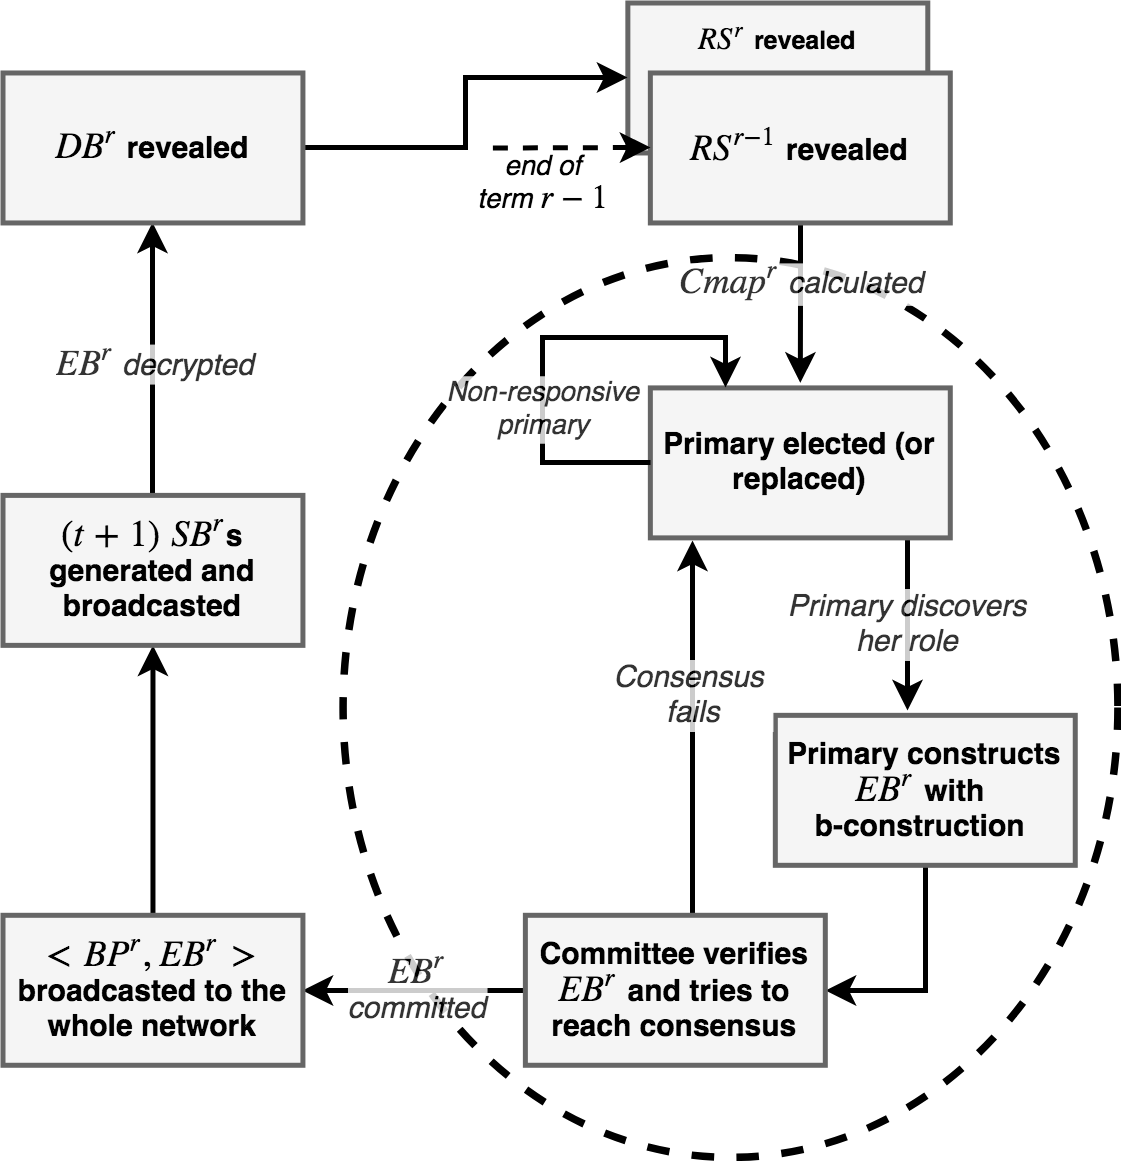
\includegraphics[width=8cm]{Helix_flow.png}
\caption{A high-level, system-view of the dynamics of a \name term. Segment four and the intra-committee communication related to the base agreement protocol lies in the dotted ellipse.}
\label{term_flow}
\end{figure}

\subsubsection*{Segment 1---Initial setup}
Since Helix relies on a threshold cryptosystem, an initial interactive step for key generation is required. A distributed key generation (DKG) protocol among the nodes would be used (e.g.,~\cite{Shoup-Gennaro, Boldyreva, NoLeaderThersholdDK2001}).

\underline{Threshold encryption}. 
We use the DKG to generate a common public key ($PK$), secret keys $(S_0,...,S_{n-1})$ and verification keys $(V_0,...,V_{n-1})$. The $PK$ is known to all entities in the system and is used to encrypt transactions. The secret and verification keys are kept privately by the nodes and are used to decrypt $etx$s. In this article we assume static membership of nodes\footnote{An interesting topic for future investigation is removing the need to redo the setup process every time a node joins or leaves. A possible approach is to generate extra key pairs and distribute them among the nodes according to some secret sharing scheme. When a new node joins she collects enough shares to construct her key pair, in the spirit of~\cite{NoLeaderThersholdDK2001}. Supporting removal of nodes can be more tricky.}.

\underline{Random seed}. 
In every term, a random seed is generated as part of the decryption of the committed Eblock. The initial random seed $RS^0$  is hard-coded into the genesis block. The initial seed will be used to determine the first Cmap and in particular the first committee.
Instead of using a dealer, a (Public)-VSS Coin Tossing scheme can be used to generate $RS^0$~\cite{SCRAP}.

\subsubsection*{Segment 2---$\pmb{etx}$ propagation}
Transactions are issued by users; each user signs and then encrypts each transaction that he issues\footnote{The choice to have users sign and then encrypt transactions favors user's anonymity, but exposes the network to spam attacks. Under our model assumptions, these attacks are mitigated by the nodes, where each node is responsible for her users. As a matter of fact, the bare minimum required is a mechanism that reveals the owner nodes of committed transactions. If this cannot be achieved in a real deployment system, user anonymity can be given up.}. Each user’s unique $sk$ is used for signing, whereas the common $PK$ is used for encryption. The $sk$ is generated locally by each user, whereas the $PK$ is hard-coded into the genesis block\footnote{To address cases in which the $PK$ changes due to a reconfiguration of the participating nodes, it is necessary to have a safe means for updating the users. We leave this discussion for future work.}. After signing and encrypting is complete, the user sends the $etx$ to his owner node.

\underline{Communicating Encrypted-transactions}.
As described previously, each $etx$ is sent by the issuing user to his owner node. The owner node then forwards the $etx$ to all the nodes in the network. A key objective of the forwarding scheme is to reduce the ability of other nodes to identify the original sender node (a node should only certify which $etx$s she owns but will not publicize this until after the Eblock containing her $etx$ is committed). This is crucial for maintaining fairness (as described in Sec.~\ref{section_properties_fairness}). Each node maintains her own Epool by adding new $etx$s she receives and by removing committed $etx$s (i.e., $etx$s included in committed Eblocks). We emphasize that the progress of segment 2 is independent of the advancement of the blockchain as described in segments 3 and 4. 

%user process
\begin{algorithm}
\caption*{\textbf{Process User}}\label{Process:User}
\begin{algorithmic}[1]
	\small
    
    \Statex \text{\fontshape{ui}\selectfont Let $sk$ be the user's secret key and $PK$ the network's }
     \Statex \text{\fontshape{ui}\selectfont public key.}
	%\State \text{\textbf{Input:} Secret key $sk$, public key $PK$ } \textit{// Issuing transaction and sending it}
    \Statex   
	\Indent
    	\Statex \textit{// Issuing transaction and casting it}
		\State $tx \gets \text{IssueNewTransaction}\big(\big) $
		\State $\sigma \gets \text{SignTransaction}\big(tx, sk\big) $  
		\State $etx \gets \text{EncryptTransaction}\big(\langle tx \rangle _{\sigma}, PK\big) $
		\State \text{Unicast\big($etx$\big)} \Comment{to owner node}

	\EndIndent

\end{algorithmic}
\end{algorithm}

\subsubsection*{Segment 3---Spreading consensus}
\label{segment3}
The main purpose of this segment is to update all non-committee members as to the consensus result from the previous term and to kick-start the next one.    

\underline{Eblocks and Block-proofs}.
In a certain term $r$, once the consensus procedure for $EB^r$ has concluded and some committee member has built a valid $BP^r$, the pair $\langle EB^r, BP^r \rangle$ should be propagated to the whole network as rapidly as possible. Once a non-committee member receives the pair $\langle EB^r, BP^r \rangle$, she performs a \emph{brief-validation} and appends $EB^r$ to her blockchain. A brief-validation of a pair $\langle EB^r, BP^r \rangle$ includes the following checks: 
\begin{enumerate}
\item The Cmap appearing in $EB^r$'s header matches the one calculated locally by the node. In particular, a correct node would refuse to append $\langle EB^r, BP^r \rangle$ unless she had already appended the previous Eblock and can calculate the current Cmap and the current committee's composition.  As a matter of fact, this step can be dropped as we explain in Sec.~\ref{section_syncs}.
\item $BP^r$ serves as a valid proof that the base agreement protocol has been carried out successfully (as described in segment four) by the rightful committee (i.e., all signers appearing in $BP^r$ appear in Cmap$^r[0,\dots,m-1]$). 
\end{enumerate}

%Since the correct committee members should have already heard of the current Eblock and independently constructed (or are in the process of constructing) the corresponding $BP$ (as explained in sec.~\ref{layer4}), it makes more sense to first propagate them to the non-committee members. This corresponds to the instructions of the communication protocol in this case.

\underline{Shares-blocks and decryption}.
As briefly noted above, Shares-blocks are constructed by nodes that have committed an Eblock and have not yet received $t+1$ Shares-blocks for that Eblock (this condition is set to reduce the number of Shares-blocks propagating in the network). Normally, committee members would be first to hear of new committed Eblocks and would thus be the ones producing Shares-blocks (this however strongly depends on message propagation in the network). After a node assembles a Shares-block, she broadcasts the Shares-block to all nodes through the fast forwarding scheme. Once a node obtains $t+1$ Shares-blocks for a committed Eblock, the Eblock is decrypted and the Dblock is revealed. We note that from the nature of the threshold encryption scheme, any valid $t+1$ Shares-blocks would produce the same Dblock. The choice $t=f$ minimizes the time from committing an Eblock to decrypting it, while maintaining \nameNS's resilience to $f$ Byzantine (and cooperating) nodes.

% Node process
\begin{algorithm} [htbp] \caption{\label{proc} \textsc{ProcessNode }} 
	\caption*{\textbf{Process Node} (for node $i$)}\label{Process:Node}
	\begin{algorithmic}[1]
    
    	\small

    	% Node's state
        \Statex \text{\fontshape{ui}\selectfont Let $r$ be the term number and $Cmap^r$ the Cmap of term $r$.}
		%\State \text{\textbf{State:} Term $r$, Cmap $Cmap^r$,}      
        
        \Statex    
        % Wait and Decrypt
        \State \text{Upon receiving a briefly validated $\langle EB^r$, $BP^r \rangle$ and $t+1$ $SB^r$s} 
            \Indent
            	
                \State \text{$DB^r \gets $DecryptEblock\big($EB^r$, $SB^r[0,\dots ,t]$\big)}
                \State \text{AppendToBlockchain\big(\big[\footnotesize $EB^r$, $SB^r[0,\dots ,t]$, $BP^r$,$DB^r$\big]\big)}
                \State \text{$Cmap^{r+1} \gets $UpdateCmap\big($DB^r$, $Cmap^{r}$\big)}
                \State $r \gets r+1$
                \State Broadcast$\big( \langle EB^r$, $BP^r\rangle \big)$
                \State \text{If $i \in Cmap^r[0,\dots ,m-1]$}
        		\Indent
                	\State \text{Trigger Process PBFT}
				\EndIndent
            \EndIndent       
	\end{algorithmic}
\end{algorithm}


\subsubsection*{Segment 4---Base agreement protocol}
\label{segment4}
Generally speaking, the base agreement protocol is a single-value variant of PBFT, re-instantiated every term, and responsible for intra-committee consensus regarding the current term's Eblock. The ellipse in Fig.~\ref{term_flow} illustrates segment four within the \name protocol. PBFT, as a Byzantine agreement protocol, enables \name to reach finality, i.e., no two correct nodes ever commit different Eblocks in the same term, as long as the bound $f$ on the number of Byzantine nodes holds (see proof in Sec.~\ref{section_properties_safety}). To emphasize this, \name inherits PBFT's robust safety guarantees---safety is kept even during times the communication network is asynchronous or unreliable. We split the segment's description into two parts. First, we describe segment four as an \emph{ideal agreement protocol} that achieves certain properties. Then, we explain how PBFT is used to implement it.  

\underline{Ideal agreement protocol}. 
The ideal agreement protocol run between $m$ nodes $u_{0},\dots,u_{m-1}$ shall implement the following primitive.
\begin{definition}[ideal agreement protocol]\label{Protocol:BBP}
An agreement protocol is said to implement the ideal agreement protocol for \nameNS's segment four if it satisfies the following properties:
\begin{itemize}
\item Validity. If a correct node commits a value $\alpha$ then some node proposed $\alpha$.
\item Liveness. If all correct nodes initiated the protocol then all correct nodes commit a value.
\item Safety. If a correct node commits a value $\alpha$ then every correct node commits $\alpha$.
\item Verifiability. If a correct node commits a value $\alpha$, then she can produce a proof $p_{\alpha}$, such that anyone can efficiently verify that $\alpha$ was agreed upon by the $m$ nodes.
\end{itemize}
\end{definition}
A typical Byzantine agreement (BA) protocol satisfies the first three items. Nodes that have not participated actively in the BA and wish to commit the agreed-upon value after the fact can do so (safely and efficiently) using the verifiability proof. 
%Verifiability allows anyone to certify the output was indeed agreed by the m participating nodes thus it implies acquaintance, i.e., the verifier must know the participating node prior the verification.realized
\nameNS's base agreement protocol implements the ideal agreement protocol, where $EB^r$ is the value agreed upon and $BP^r$ serves as a proof that it was indeed agreed upon by nodes $u_0,\dots,u_{m-1}$. The question remains though---which nodes are the rightful committee members in term $r$? In order to avoid forks (i.e., inconsistencies), \name must figure out a way for all the participating nodes to come to an agreement as to a single committee. This is done using $EB^{r-1}$ which contains a commitment to the seed that determines the $r$-term committee. Using an inductive argument, if there are no forks in term $r-1$, then only a single committee is possible in term $r$ and accordingly there can neither be forks in term $r$. Finally, since the first committee is hard-coded into the genesis block and agreed upon by all nodes, \name enjoys no forks. 

\underline{Simplified PBFT as the ideal agreement protocol}.
In \nameNS, the ideal agreement protocol is implemented using a simplified version of PBFT~\cite{PBFT} that reaches agreement over a single value. We assume a familiarity with PBFT's logic and terminology and describe Helix's adjustments and modifications to PBFT\footnote{To keep our presentation concise, we leave PBFT's original point-to-point communication intact and do not adopt a more bandwidth-economical protocol such as CoSi~\cite{CoSi} as proposed in Byzcoin~\cite{Byzcoin} or Zilliqa~\cite{Zilliqa}. In \nameNS, optimizations to PBFT's bandwidth consumption can be relieved as we assume $m \ll n$, where $m$ is the size of the committee running PBFT.}.

\textit{Accepting an Eblock}. \label{Protocol:ValidateEB}
In PBFT, a node \emph{accepts} a pre-prepare message (and the value she proposes) by broadcasting a corresponding prepare message after validating the following: 
\begin{enumerate}
\item The view in the pre-prepare message matches her internal view number.
\item The pre-prepare message is signed by the rightful primary in that view.
\item She has not accepted a pre-prepare message in the same view containing a different Eblock.
\end{enumerate}

In \nameNS, when accepting $EB^r$, a correct committee member further validates that:
\begin{enumerate}
\item $EB^r$'s header contains Cmap$^r$ as locally computed with $DB^{r-1}$ and $EB^{r-1}$. We emphasize that a correct committee member does not depend on $EB^r$'s header in order to figure out whether she is in the committee or not. This implies that in order to participate in a committee a correct node must obtain $DB^{r-1}$ and $EB^{r-1}$.
%A correct committee member also checks it appears somewhere in the first $m$ places in Cmap$^r$. 
%(for $RS^{r-1}$ which depends on $MDR^{r-1}$, and the new reputations which can be calculated from the old ones (that appear in Cmap$^{r-1}$), the composer of $EB^{r-1}$ and the view in which it was committed locally for the first time. All these are written in the header of $EB^{r-1}$).
\item $EB^r$'s header contains a valid hash pointer to $EB^{r-1}$.
\item $EB^r$'s header contains a valid hash pointer to $DB^{r-1}$.
\item $EB^r$'s header contains a valid hash of concatenated $ese$s, i.e., $H(ese^r_{i_0},\dots,ese^r_{i_{t}})$, properly signed by the different nodes $i_0,\dots,i_{t}$ (taken from the $t+1$ $SB^{r-1}$s the composer node used in order to decrypt $EB^{r-1}$).
\item $EB^r$'s header contains the correct composer and view (this can be validated with the new-view messages, if exist).
\item $EB^r$'s payload contains at most $b$ $etx$s.
\end{enumerate}

\textit{View-change mechanism}. 
In PBFT, when timeouts expire (e.g., due to a faulty primary or an unexpected network slowdown) view-change messages are broadcasted with the aim of replacing the primary. In order to ensure safety is maintained cross-views, proofs of previously committed values are submitted within the view-change mechanism. To avoid rerunning all the committed values from the beginning of time, a checkpoint mechanism is introduced where proofs are sent only for values that were committed after the last stable checkpoint. 
\nameNS's blockchain construction enables invoking a new instance of a single-value PBFT for each term (this single-value PBFT implements the ideal agreement protocol). Thus, the checkpoint and truncating mechanism can be given up altogether (while primaries keep being replaced seamlessly). In addition, new-view messages contain only one pre-prepare message which never contains the null digest, $d^{null}$. Only in case a new Eblock is proposed, the Eblock itself is passed as regularly done with pre-prepare messages.

\textit{Verifying consensus}.
The verifiability property of the ideal agreement protocol (see definition~\ref{Protocol:BBP}) is obtained by the Block-proof that stores a signed pre-prepare message, $2f$ corresponding signed prepare messages and $2f+1$ corresponding signed commit messages\footnote{We note that in order to reduce the size of such a proof, aggregation of signatures or a threshold signature scheme may be deployed, as in~\cite{Hot-Stuff}.}. On its own, a Block-proof is not enough as a node needs to know the composition of the term's committee and make sure all the signers are indeed committee members. As mentioned before, this can be deduced from the previous term's block. We show in Sec.~\ref{section_properties_safety} that $BP^r$ indeed serves as an unforgeable proof a $EB^r$ was committed-locally by some correct committee member in term $r$. Thus, the pair $\langle EB^r, BP^r \rangle$ (after validation) is safe to append to one's blockchain.

\textit{Timeout mechanism}.
We consider two timeout mechanisms for \nameNS. In PBFT's original approach, timeouts are deterministic and double every time the view increases, i.e., the timer in view $v$ is set to be $2^{v-1} x$, for some positive value $x$. This ensures that in a timely network, all backups will eventually converge to a specific view (that of the current most advanced backup or one view later), even if the network performs unreliably for a restricted amount of time. This technique, although it works in theory, is very problematic (see ~\cite{Prime}) as timeouts must keep growing and cannot be adjusted to be shorter\footnote{As a matter of fact, once a backup commits-locally a value in PBFT, she could potentially start over with timer set to $x$ in the next view, leaving in previous views at most $f$ backups. These would eventually be synced with the checkpoint mechanism.}.

We suggest a different possible timeout mechanism, in which timeouts remain constant and thus highly relies on the network being reliable and predictable in latency. Every time an instance of PBFT is initiated, or when a view-change message is sent, a node's timer is reset to the same value, $x = \max \left\{ 2\Delta, \text{ } \Delta+3\delta \right\}$. In a nutshell, this value is set so that it expires only after a committee member is certain a correct primary had enough time to get her Eblock committed. In the next section, we prove formally that \name is indeed live under the condition any piece of information a node broadcasts (according to the fast forwarding scheme) is received by all correct nodes within a known bound $\Delta$ (see App.~\ref{appendix_comm} that discusses \nameNS's communication schemes).    

%AVI: add highest view value in the NEW-VIEW message....
%Process PBFT
\begin{algorithm*}
	\caption*{\textbf{Process PBFT} (for committee member $i$)}\label{Process:PBFT}
	\begin{algorithmic}[1]  
    	%\algsetup{linenosize=\tiny}
    	\small
        
        
    	\Statex \text{\fontshape{ui}\selectfont Let $r$ be the term's number, Cmap$^r$ the Cmap of term $r$, $v \in \mathbb{N}$ the view, and $CEB$ a candidate Eblock.}
        \Statex \text{\fontshape{ui}\selectfont Let $j \in $Cmap$^r [\,0,\dots,m-1]\,$ be a committee member and $p_v=$Cmap$^r[\,v~mod~m]\,$ be v's primary.}
		%\State  \text{This process is triggered by DecryptProcess.} 
        %\State $\textbf{Input: } \text{Term $r$, Cmap $Cmap^r$. } $
        \Indent
        %\State \textbf{Def: }\text{Let $j \in Cmap^r [\,1,\dots,m]\,$ be a committee member and $p \in Cmap^r[\,1]\,$ be the primary.}
        
       \Statex
		%\Procedure{BackupProcess$\left(Cmap^r,\text{ } r \right)$ }{}
        \Statex \textbf{Init: } \text{$v \gets 0$, $CEB \gets null$, $prepared \gets false$, $committed\_locally \gets false$, $\mathcal{P}_i^r \gets null$.}
        \Statex \textbf{Timer: } \text{Set timer to $x_0=x$ and start countdown.}
        
        \Statex
        
        \Statex \textit{// First primary}
        \State \text{If $i=p_0$,} 
            \Indent
                \State $CEB \gets \text{ConstructEblockFromEpool\big(\big)}$
                \State \text{Multicast$_{committee}$\big($\big\langle\langle \text{PRE-PREPARE, $0$, $r$, H}(CEB)\rangle _{\sigma_{p_0}} \text{, }CEB \big\rangle$\big)}
            \EndIndent
        
        \Statex
        	\Statex \textit{// Normal flow}
            \State $\text{Upon receiving a } \big\langle\langle \text{PRE-PREPARE, $v$, $r$, H}(EB)\rangle _{\sigma_{p_v}} \text{, }EB \big\rangle \text{ message}$
            
            \Indent
                \State \text{ValidateEblock$\big(EB \big)$}  \Comment see Sec.\ref{Protocol:ValidateEB}
                \State $CEB \gets EB$ 
                \State \text{Multicast$_{committee}$\big($\langle \text{PREPARE, $v$, $r$, H}(CEB) \text{, }pk_i\rangle _{\sigma_i}$\big)} 
            \EndIndent

            \State $\text{Upon receiving $2f$ }  \langle \text{PREPARE, $v$, $r$, H}(CEB) \text{, }pk_i\rangle _{\sigma_j} \text{ messages and } CEB \neq null   $ \label{PBFT:Backup:Primary_Join}
            \Indent
                \State $prepared \gets true$
                \State \text{Multicast$_{committee}$\big($\langle \text{COMMIT, $v$, $r$, H}(CEB) \text{, }pk_i\rangle _{\sigma_i}$\big)} 
            \EndIndent

             \State $\text{Upon receiving $2f+1$ } \langle \text{COMMIT, $v$, $r$, H}(CEB) \text{, }pk_i\rangle _{\sigma_j} \text{ messages and } prepared = true$
            \Indent
                \State $committed\_locally \gets true$
				\State $BP \gets \text{ConstructBP\big(\big)}$
                \State \text{PropagateEB\big($  CEB$, $BP$\big)}
            \EndIndent
            
            \Statex 
            \Statex \textit{// Timeout: primary change proposal}
            
            
            
            \State \text{Upon timer expiry, reset timer to $x_{v+1}=2^{v+1} x_0$}
            \Indent
            	\State \text{$\mathcal{P}_i^r = null$}
            	\State \text{If $prepared=true$ then,}
                \Indent
                	\State \text{$\mathcal{P}_i^r = \begin{cases}
       \mathcal{P}_i^r.EB \gets CEB\\
       \mathcal{P}_i^r.msgs_v \gets 2f+1\text{ PREPARE messages with view $v$, received for $CEB$}\\
     \end{cases}$}
                \EndIndent
                \State \text{Unicast$_{p_{v+1}}$\big($\langle \text{VIEW-CHANGE, $v+1$, $r$, $\mathcal{P}_i^r$, } pk_i\rangle _{\sigma_i} $}\big) 
                \State $v \gets v+1$
            \EndIndent
            
            \Statex 
            \Statex \textit{// Primary change takeover, for $p_{\tilde{v}}$}
            
            \State \text{Upon receiving $2f+1$} $\langle \text{VIEW-CHANGE, $\widetilde{v}$, $r$, $\mathcal{P}_j^r$, } pk_j\rangle _{\sigma_j} $ \text{messages, denote them by $\mathcal{V}$}
            \Indent
            	%\State \text{$\mathcal{V} \gets 2f+1$ view-change messages received}
            	\State \text{If there exists a $j$ s.t. $\mathcal{P}_j^r \neq null$ then, } 
                \Indent
                	\State \text{$j \gets$ the node with the maximal $v$ among $\mathcal{P}_j^r.msgs_v$}
                	\State \text{$CEB \gets \mathcal{P}_j^r.EB$}
                \EndIndent
                \State \text{Otherwise,}
                \Indent
                	\State \text{$CEB \gets$ ConstructEblockFromEpool\big(\big)}
                \EndIndent
                \State \text{$\mathcal{O} \gets \big\langle\langle \text{PRE-PREPARE, $\widetilde{v}$, $r$, }H(CEB)\rangle _{\sigma_i} \text{, }CEB \big\rangle$}
                \State \text{Multicast$_{committee}$\big($\langle \text{NEW-VIEW, $\widetilde{v}$, $r$, $\mathcal{V}$, $\mathcal{O}$}\rangle $\big)} \Comment{NEW-VIEW messages, after validated, are treated as} \par
                \Comment{PRE-PREPARE messages by recipients}
            \EndIndent

        \EndIndent     
	\end{algorithmic}
\end{algorithm*}

%\red{Note (terminology): a committed Eblock is an Eblock that was committed locally by at least one correct node and thus has a valid block-proof. It is also guaranteed to be the next Eblock appended to the blockchain.}


%add the partial synchrony timeout scheme and explain why necessary.
%Some terms may be very quick while others might take longer.

\subsection{Incentive mechanism in \nameNS}
\label{Reputation} 
%\red{Looks good. I would just make some changes in the presentation: I think we should start with the fact we want to incentive some behaviors, then present fees (explaining they are paid by nodes to nodes) and reputation (explaining again their influence). We can then give the list of examples, and then refer to the calculation of their inputs.}
Processing a transaction in \name costs money as it consumes resources such as bandwidth, storage and computation. Each node is responsible for the processing costs of transactions issued by her own users\footnote{The way a node covers the costs of her users depends on her business model, e.g., funding may come from the users themselves or from a third party.}. However, the cost for processing transactions for other nodes’ users may be considerable, and thus requires in-protocol compensation from those nodes. If all nodes produce the same amount of transactions, compensation is settled trivially as costs balance. Though if nodes produce different amounts of transactions, a fee mechanism that offsets costs among nodes is required. Fees would basically be paid by nodes with a high transaction rate to those with a low transaction rate\footnote{At this point we do not elaborate as to the implementation of \nameNS's fee mechanism, but assume that the fee is proportional to a node's transaction rate.}. 

Fees, in addition to balancing costs, serve as means to incentivize nodes to follow the protocol's instructions and allow the protocol to reach optimal performance. This is achieved by a reputation score that is attributed to each node and is updated frequently. The reputation strives to serve as a reliable measure to a node's quality of service. A node’s reputation is taken into account when calculating her fee tariffs, where nodes with low reputation can charge lower fees for their services than their peers, possibly resulting in losses. For this reason, it is important that both the measurement of the resource usage and of the quality of service are accurate. %(or: resources and behavior)

%Gruffalo's fee mechanism is based on a trusted third party\footnote{This entity can be represented by a smart contract\red{, in a different platform or over Gruffalo itself}.} that collects fees from nodes and pays them back later taking into account their issuance rate and reputation. In practice the third party would transfer funds from nodes with high usage to those with low usage taking into account nodes' reputation. Nodes with low reputation will be paid back less than their relative share, resulting in losses. Thus, it is crucial that Gruffalo's fee mechanism will measure accurately the usage of each node and that the reputation will measure correctly nodes' resources and behavior.

Measuring a node's usage is straightforward after revealing the owner nodes of all $etx$s in the decryption process. Making sure the reputation is consistent with \nameNS's requirements and instructions is more complicated. We suggest a few practical criteria that the reputation may examine, but a more elaborate discussion as to its exact specification is due at a later time. We further note that with the evolution of the system, the reputation measure may be enhanced to mitigate new found vulnerabilities in the protocol or to encourage new desired behaviors. The discussion above makes clear that nodes are incentivized to increase their reputation, but also wish to include their own $etx$s in Eblocks as fast as possible. These two distinct preferences may be conflicting, requiring nodes to prioritize.

We shall now illustrate a naive reputation measure. It is updated frequently (e.g., every 1000 blocks or every month), locally and deterministically by each node, according to the blockchain. A few concrete examples:
\begin{itemize}
\item In order to make sure that nodes maintain high uptime and stay available, every node is evaluated according to the average view number of committed Eblocks when she was a committee member. The higher the average view, the lower the reputation should be.
\item In order to make sure that nodes maintain the recent blockchain history, if an Eblock consists of a previously included $etx$, its composer should be punished by reducing hers reputation.
\item In order to make sure that nodes select $etx$s randomly (see Sec.~\ref{section_highload} for more details), adjacent Eblocks should represent similar distributions (in terms of the owner nodes of the $etx$s they include). If a specific node is found to construct Eblocks that significantly deviate from the Eblocks in their surrounding, she should be penalized by reducing her reputation.
\item In order to encourage nodes to stay up-to-date with protocol changes, a node that constructs an Eblock with a decommissioned protocol version should be penalized by reducing her reputation.
\end{itemize}

We emphasize that the reputation update rules that do not depend on Dblocks may be used as validation checks in the agreement protocol. On the contrary, some of the validation checks in Sec.~\ref{Protocol:ValidateEB} may be relaxed and become a part of the reputation mechanism. %These two mechanisms share a common goal---to have the blockchain represent nodes' needs and desires. 
An interesting possibility is to relate reputation to a node's stake in the system. We also note that the reputation measure is shared across other services in the system such as the execution service.

